\chapter{Introduction}

\section{Context}

Bone is irrigated by a dense network of blood vessels, and osteoarthritis is thought to change it.
In 2017, the SAINBIOSE laboratory (U1059, Saint-Étienne) was studying these changes in animal models:
the researchers injected a radio-opaque contrast agent (barium sulfate) into the circulation of mice,
then imaged the knee by micro-computed tomography ($\mu$CT, GE Nanotom). The barium makes the vessels
visible to X-rays, but no software was dedicated to measuring a \emph{vascular} network inside bone:
the tools they had were made for bone histomorphometry.

The laboratory proposed the problem as a final-year project at CPE Lyon (5ETI -- IMI major,
2017--2018), and I was one of the four students who took it on. The brief was to separate the vascular
network from the bone tissue, reconstruct it in 3D and, in the longer run, quantify it (number of nodes
and branches, vessel calibre, branch lengths). In a few weeks we delivered a Matlab segmentation and a
Python viewer, which the researchers approved. Chapter~\ref{chap:legacy} summarises what we did.

Looking back at it eight years later, I find our approach naive: every parameter was a pixel count tuned
by eye on a single scan, and nothing told us whether a change made the segmentation better or worse.
I wanted to know how far the same problem could be taken with a clean method, so I rewrote the project
from scratch. This report covers that rewrite, \textbf{pyBones}. I set myself four goals at the start:
\begin{itemize}
  \item no Matlab: Python only, with a minimal set of dependencies (numpy and OpenCV for the
        computations, pydantic for the configuration, scikit-image for marching cubes only; later,
        FastAPI and uvicorn for the web server, three.js, kept in the repository, for the page, and
        scikit-image's 3D skeletonisation and SciPy for the vascular quantification);
  \item clean, documented, tested code, every tunable value in a validated configuration file;
  \item computation speed and memory as first-class concerns, but correctness first;
  \item improve the results, and \emph{prove} it.
\end{itemize}

\section{The data}

The only dataset I have is a stack of 100 slices of a mouse knee: the distal femur on top, the proximal tibia
below, the joint and menisci in between (Figure~\ref{fig:overview-raw}). Each slice is a
$2300 \times 1487$ 16-bit image; the stack weighs about 685\,MB. The 2018 project used a slice
thickness of 3\um; I assumed isotropic 3\um{} voxels, which gives anatomically consistent sizes
(a knee about 3\,mm wide, a femoral cortex about 165\um{} thick).

Three kinds of material appear, from dark to bright:
\begin{itemize}
  \item soft tissue and marrow (background), mean intensity \pbValueMeanBackground;
  \item \bone{} (cortex and trabeculae), mean \pbValueMeanBone;
  \item barium-filled vessels, mean \pbValueMeanVessel, and much brighter clusters where the contrast
        agent leaked out of vessels. The researchers had told us that the knee went through a freezer:
        ice can rupture vessels, and blood can clot inside them. The leaked clusters are labelled
        \burst{}; clotted vessels appear as dim, partially filled \vessel{} segments.
\end{itemize}

\begin{figure}[ht]
  \centering
  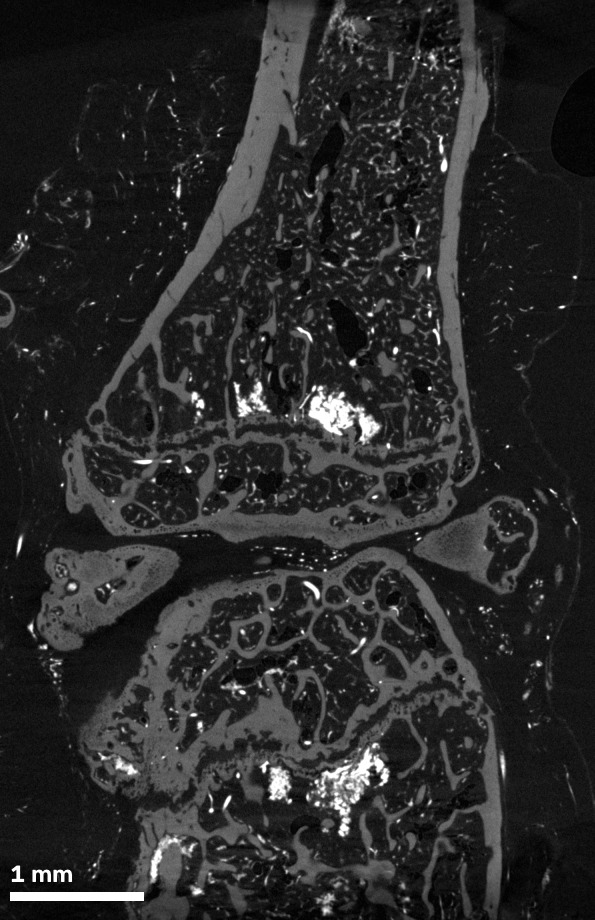
\includegraphics[width=0.48\linewidth]{overview_raw.jpg}
  \caption{Slice 0 of the stack (contrast-stretched). Femur on top, tibia below. The bright white
    clusters inside the bone are bursts of contrast agent; the bright threads are vessels.}
  \label{fig:overview-raw}
\end{figure}

\section{Structure of this report}

Chapter~\ref{chap:legacy} summarises the 2018 project and its limitations. Chapter~\ref{chap:rewrite}
presents the architecture of the rewrite, its web server and the page that replaces our 2018 viewer. Chapter~\ref{chap:segmentation} explains each step of the
segmentation, why I built it that way, and what it changed. Chapter~\ref{chap:validation} shows how I
validated the results without any expert annotation, and how every intermediate version of the
rewrite scores on the same synthetic ground truth. Chapter~\ref{chap:performance} covers speed and
memory, Chapter~\ref{chap:limitations} what is still out of reach, and Chapter~\ref{chap:conclusion}
concludes. Appendix~\ref{chap:reproduce} lists the commands that reproduce every figure and number.

\begin{keypoint}
Every measured value quoted in this report (thresholds, scores, timings, and the machine they were
measured on) is generated by \code{python -m tools.report} from the data and the git history; none
of them is typed by hand.
\end{keypoint}
